\documentclass{article}
\usepackage{graphicx}
\usepackage{multicol} % use to multiple column in itemize
\usepackage{float}
\usepackage{setspace}
\setlength{\parskip}{0.5em}

\begin{document}

\title{Linear Regression}
\author{Cong Cuong PHAM}

\maketitle

\begin{abstract}
This document introduces some fundamental notions of Linear Regression.
\end{abstract}

\section{Introduction}
\subsection{What is Linear Regression?}
\par 1800s: Francis Galton, was studying the relationship between parents and their children. He investigated the relationship between the heights of fathers and their sons. He discovered that a man's son tended to be roughly as tall as his father. However Galto's breakthrough was that the son's height tended to be closer to the overall overage height of all people. Galton called this phenomenon {\bf{regression}}, as in ``A father's son's height tends to regress (or drift towards) the mean (average) height''.

\begin{figure}[H]
    \centering
    \begin{minipage}{.5\textwidth}
        \centering
        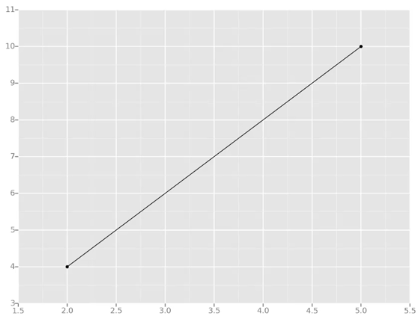
\includegraphics[width=\linewidth,height=\linewidth]{pic/two-points.png}
        \caption{Two point}
        \label{fig:two-points}
    \end{minipage}%
    \begin{minipage}{0.5\textwidth}
        \centering
        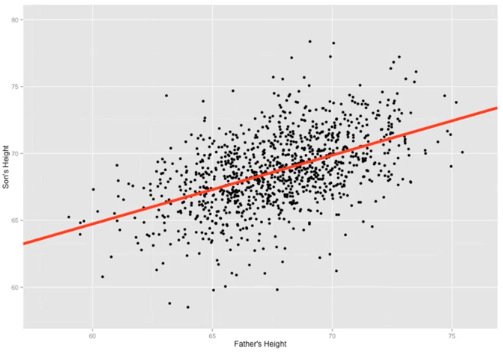
\includegraphics[width=\linewidth,height=\linewidth]{pic/multi-points.png}
        \caption{Multiple points}
        \label{fig:multi-points}
    \end{minipage}
\end{figure}

\par The goal of linear regression is to {\bf{minimize the vertical distance}} between all the data point and the fitted line. In determining the {\bf{best line}}, we are attempting to minimize the distance between {\bf{all}} the points and their distance to the fitted line \ref{fig:multi-points}.

\par There are lots of different ways to minimize the vertical distance (sum of squared errors, sum of absolute errors, etc), but all these methods have a general gold of minimizing this value. The residuals for an observation if the different between the observation (the y-value)  and the fitted line.

\par Example: Us the Least Squares Method which is fitted by {\bf{minimizing the sum of squares of the residuals}}.
\begin{figure}[H]
\centering
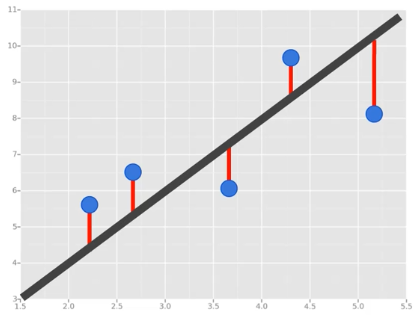
\includegraphics[width=0.6\linewidth]{pic/residuals-example.png}
\caption{Choose the fitted line by minimizing the sum of square of the residuals.}
\end{figure}

\end{document}